\chapter{Bundle Adjustment}
\label{ch:bundle_adjustment}

\section{Overview}

\newenvironment{myindentpar}[1]
               {\begin{list}{}
                   {\setlength{\leftmargin}{#1}}
                 \item[]
               }
               {\end{list}}

\definecolor{lgray}{gray}{0.95}

Satellite position and orientation errors have a direct effect on the
accuracy of digital elevation models produced by the Stereo Pipeline.
If they are not corrected, these uncertainties will result in
systematic errors in the overall position and slope of the \ac{DEM}.
Severe distortions can occur as well, resulting in twisted or ``taco
shaped'' \acp{DEM}, though in most cases these effects are quite
subtle and hard to detect. In the worst case, such as with old mission
data like Voyager or Apollo, these gross camera misalignments can
inhibit Stereo Pipeline's internal interest point matcher and block
auto search range detection.
\begin{figure}[bt]
  \centering
  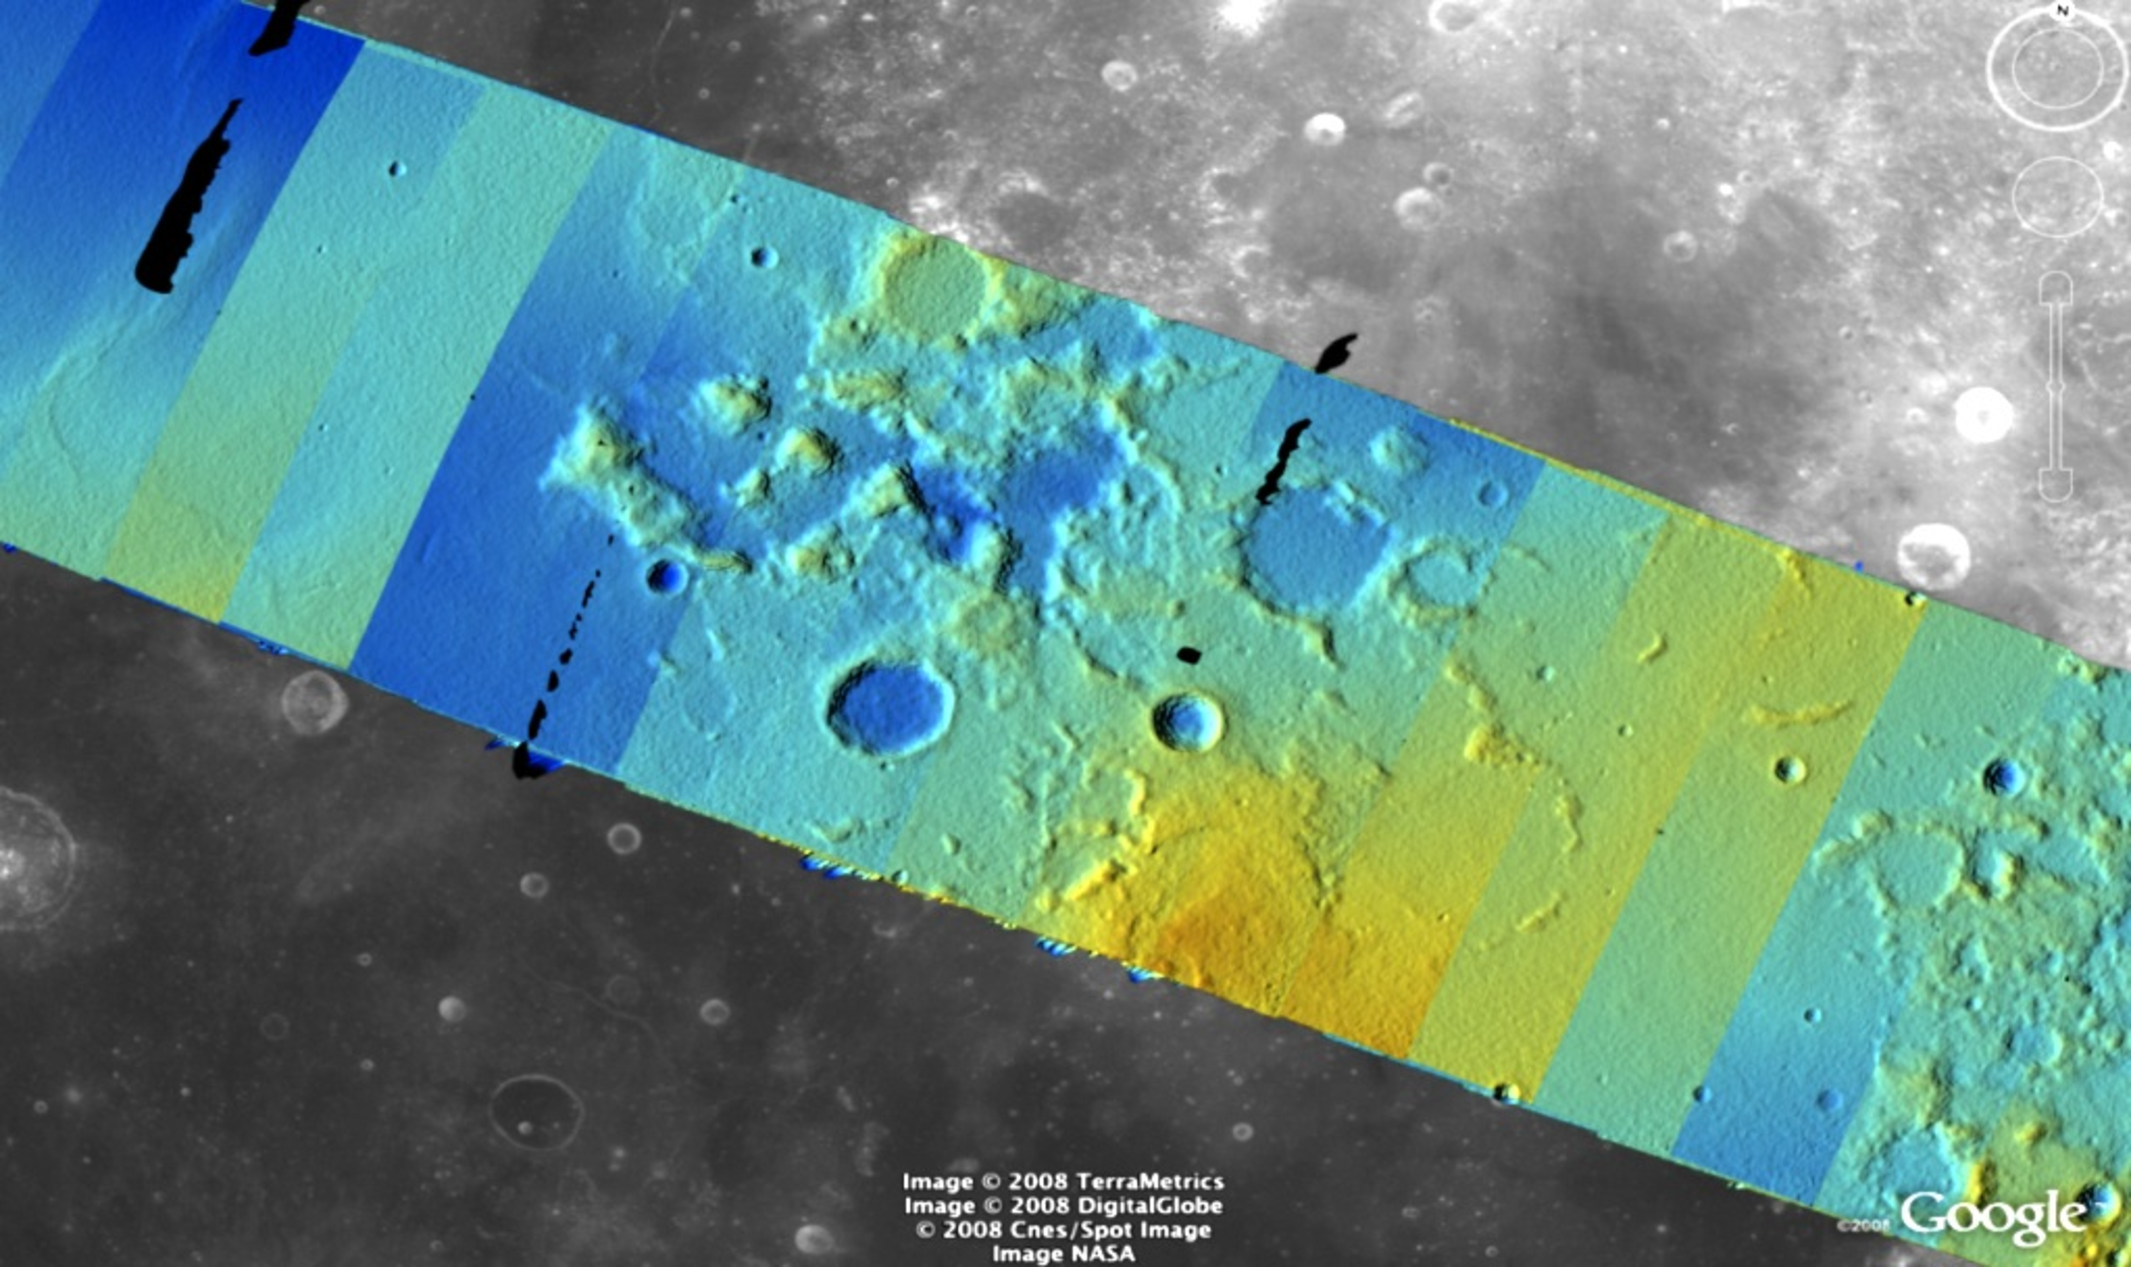
\includegraphics[width=8cm]{images/ba_orig.pdf}
  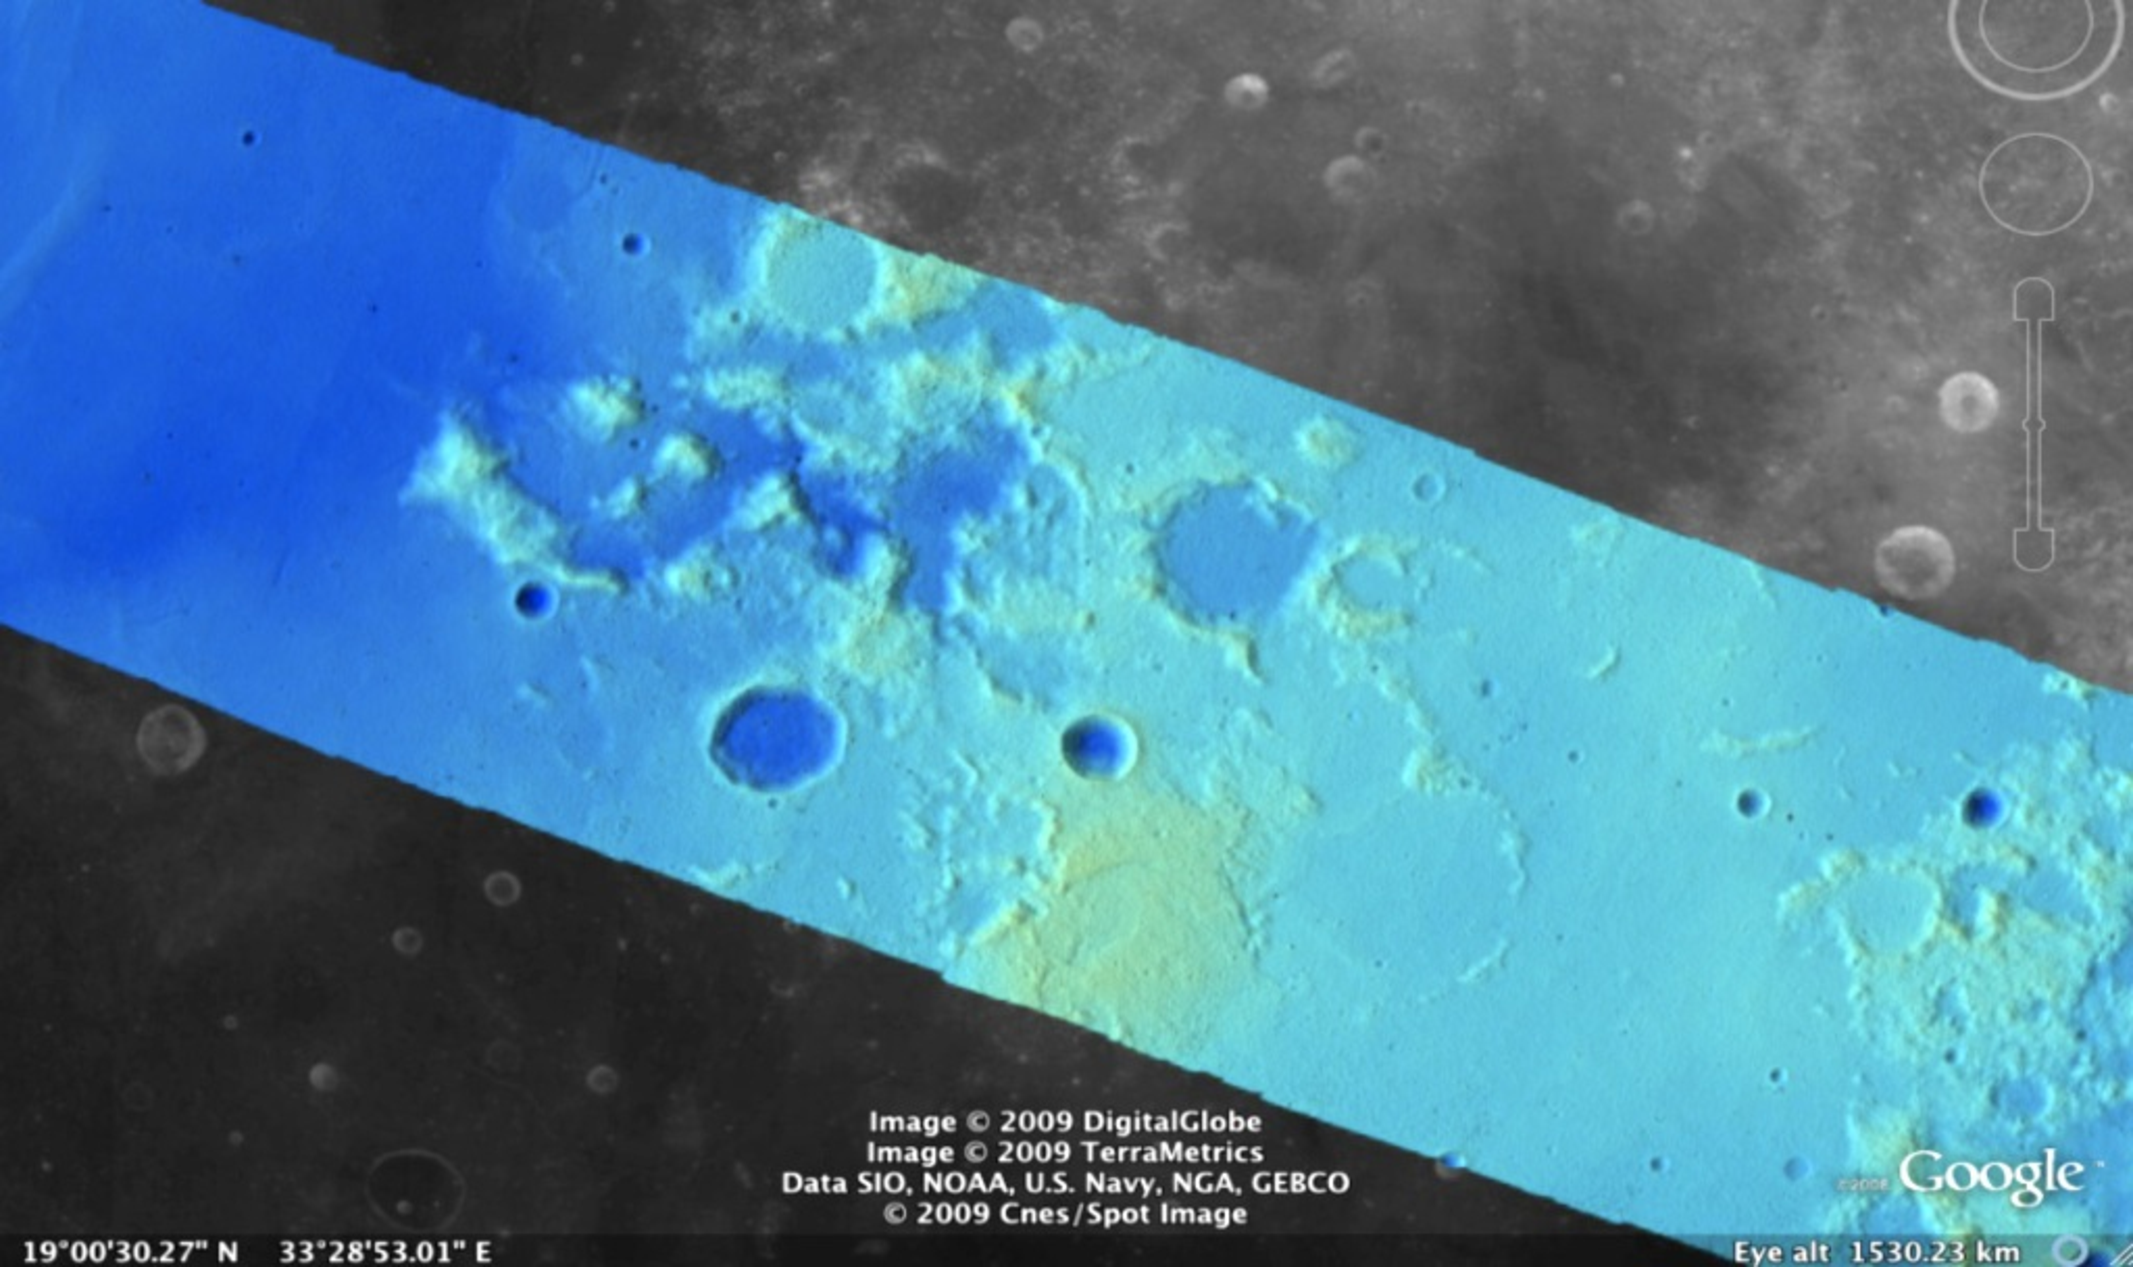
\includegraphics[width=8cm]{images/ba_adjusted.pdf}
  \caption{Bundle adjustment is illustrated here using a color-mapped,
    hill-shaded DEM mosaic from Apollo 15, Orbit 33, imagery. (a)
    Prior to bundle adjustment, large discontinuities can exist between
    overlapping DEMs made from different images. (b) After bundle
    adjustment, DEM alignment errors are minimized and no longer visible.}
  \label{fig:bundle_adjustment}
\end{figure}

Errors in camera position and orientation can be corrected using a
process called \emph{bundle adjustment}. Bundle adjustment is the
process of simultaneously adjusting the properties of many cameras and
the 3D locations of the objects they see in order to minimize the error
between the estimated, back-projected pixel locations of the 3D objects
and their actual measured locations in the captured images.

This complex process can be boiled down to this simple idea: bundle
adjustment ensures that the observations in multiple images of a
single ground feature are self-consistent. If they are not consistent,
then the position and orientation of the cameras as well as the 3D
position of the feature must be adjusted until they are.  This
optimization is carried out along with thousands (or more) of similar
constraints involving many different features observed in other
images.  Bundle adjustment is very powerful and versatile: it can
operate on just two overlapping images, or on thousands. It is also a
dangerous tool. Careful consideration is required to insure and
verify that the solution does represent reality.

Bundle adjustment can also take advantage of \acp{GCP}, which are
3D locations of features that are known a priori (often by measuring
them by hand in another existing \ac{DEM}). \acp{GCP} can improve the internal
consistency of your \ac{DEM} or align your \ac{DEM} to an existing data
product. Finally, even though bundle adjustment calculates the
locations of the 3D objects it views, only the final properties of
the cameras are recorded for use by the Ames Stereo Pipeline. Those
properties can be loaded into the \texttt{stereo} program which
uses its own method for triangulating 3D feature locations.

When using the Stereo Pipeline, bundle adjustment is an optional step
between the capture of images and the creation of \acp{DEM}. The bundle
adjustment process described below should be completed prior to
running the \texttt{stereo} command.

Although bundle adjustment is not a required step for generating
\acp{DEM}, it is {\em highly recommended} for users who plan to
create \acp{DEM} for scientific analysis and publication.  Incorporating
bundle adjustment into the stereo work flow not only results in
\acp{DEM} that are more internally consistent, it is also the correct
way to co-register your \acp{DEM} with other existing data sets and
geodetic control networks.

At the moment however, Bundle Adjustment does not automatically work
against outside \acp{DEM} from sources such as laser altimeters.
Hand-picked \acp{GCP} are the only way for \ac{ASP} to register to those
types of sources.

\section{Bundle adjustment using ASP}
\label{baasp}

Recently, Stereo Pipeline started providing its own bundle adjustment
tool, named \texttt{bundle\_adjust}. Its usage is described in section
\ref{bundleadjust}.

Here is an example of using this tool on a couple of Apollo 15 images,
and its effect on decreasing the stereo triangulation error.

\begin{figure}[h!]
\centering
  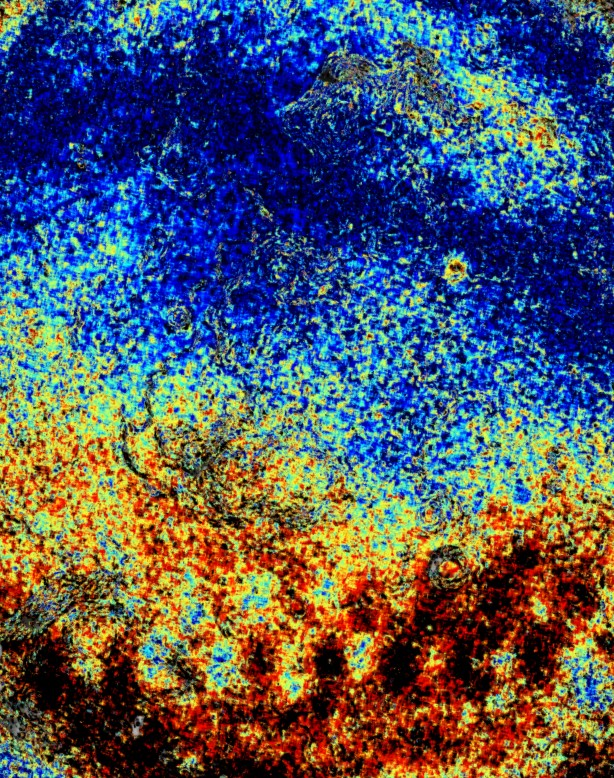
\includegraphics[width=3.0in]{images/examples/before_ba.jpg}
  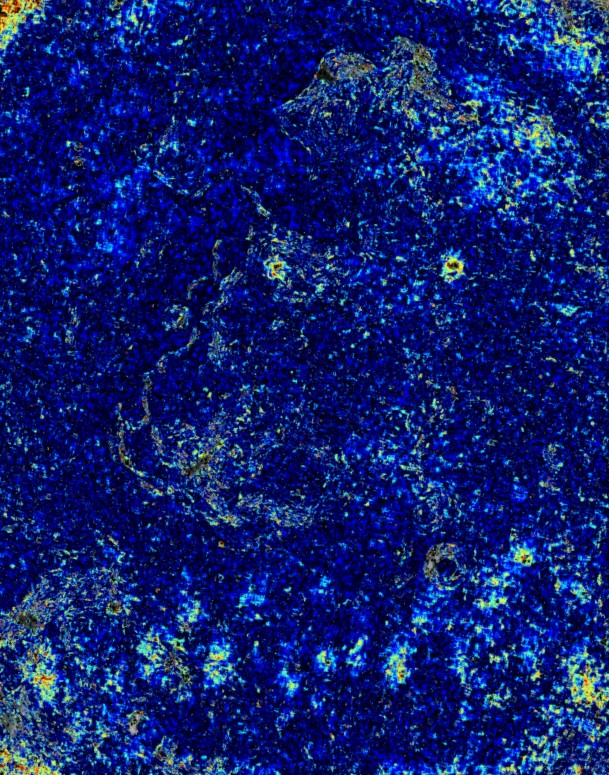
\includegraphics[width=3.0in]{images/examples/after_ba.jpg}
\caption{Illustration of the triangulation error map for a pair of
  images before (left) and after (right) using Stereo Pipeline's
  \texttt{bundle\_adjust}. Red and black colors suggest higher error.}
\label{fig:asp-ba-example}
\end{figure}

Running \texttt{stereo} without using bundle-adjusted camera models.
\begin{verbatim}
  stereo AS15-M-1134.cub AS15-M-1135.cub run_noadjust/run
\end{verbatim}

Performing bundle adjustment.
\begin{verbatim}
  bundle_adjust AS15-M-1134.cub AS15-M-1135.cub -o run_ba/run
\end{verbatim}

Running stereo while using the bundle-adjusted camera models.
\begin{verbatim}
  stereo AS15-M-1134.cub AS15-M-1135.cub run_adjust/run \
    --bundle-adjust-prefix run_ba/run
\end{verbatim}

A comparison of the two ways of doing stereo is shown in figure \ref{fig:asp-ba-example}.

\subsection{Floating intrinsics and using a lidar or DEM ground truth}
\label{floatingintrinsics}

This section documents some advanced functionality, and it suggested the
reader study it carefully and invest a certain amount of time to fully
take advantage of these concepts.

When the input cameras are of pinhole type, it is possible to optimize
the intrinsic parameters, in addition to the extrinsics. It is also
possible to take advantage of an existing terrain ground truth, such as a lidar file or a DEM,
to correct imperfectly calibrated intrinsic parameters, which can result in greatly
improved results, such as creating less distorted DEMs that agree much better
with the ground truth. 

\subsubsection{A first attempt at floating the intrinsics}

We recommend that first bundle adjustment is run with the intrinsics fixed,
to get the extrinsics mostly correct, as optimizing for both of them at
the same time may result in a non-convex problem which may lead to a 
suboptimal local minimum. Then, we will jointly optimize the intrinsics
and extrinsics. 

Note that when solving for intrinsics, \texttt{bundle\_adjust} will by default
optimize all intrinsic parameters and will share them across all cameras (which must
be the same type).  You can control this behavior with the 
\texttt{-\/-intrinsics-to-float} and \texttt{-\/-intrinsics-to-share} parameters.

Hence, the first invocation of camera optimization should be like:

\begin{verbatim}
  bundle_adjust -t nadirpinhole --inline-adjustments      \
    left.tif right.tif left.tsai right.tsai -o run_ba/run
\end{verbatim}

It is suggested that one run \texttt{stereo} with the obtained cameras, 
and then examine the intersection error:

\begin{verbatim}
  stereo -t nadirpinhole --alignment-method epipolar left.tif right.tif \
     run_ba/run-left.tsai run_ba/run-right.tsai run_stereo/run 
  point2dem --tr RESOLUTION --errorimage run_stereo/run-PC.tif
  gdalinfo -stats run_stereo/run-IntersectionErr.tif
  colormap run_stereo/run-IntersectionErr.tif
  stereo_gui run_stereo/run-IntersectionErr_CMAP.tif
\end{verbatim}

If desired, fancier stereo correlation algorithms can be used, such as MGM, as detailed in  
chapter \ref{ch:correlation}. For \texttt{colormap}, \texttt{-\/-min} and \texttt{-\/-max} 
bounds can be specified if the automatic range is too large. We also suggest inspecting
the interest points:
\begin{verbatim}
  stereo_gui left.tif right.tif run_ba/run
\end{verbatim}
and then viewing the interest points from the menu. 

If the interest points are not well-distributed, this may result in large ray intersection errors
where they are missing. If so, they can be re-created by modifying \texttt{-\/-ip-detect-method}
and \texttt{-\/-ip-per-tile}. Or, one can take advantage of the just-completed stereo run
and invoke \texttt{stereo\_tri} with the additional option 
\begin{verbatim} 
  --num-matches-from-disp-triplets 10000
\end{verbatim}

to create dense and uniformly distributed interest points with desired density
(the latter creates a .match file that needs to be copied to the name
\texttt{bundle\_adjust} expects). This option also ensures that if three
images are present, and stereo is invoked on the first and second image,
and then on the second and the third, followed by interest point generation,
many interest points will be triplets, that is, the same feature will often
will be identified in all three images, which
can be a very good constraint on bundle adjustment later.

If the interest points are good and the mean intersection error is
acceptable, but this error shows an odd nonlinear pattern, that means
it may be necessary to optimize the intrinsics. We do so by using the
cameras with the optimized extrinsics found earlier, that is:

\begin{verbatim}
  bundle_adjust -t nadirpinhole --inline-adjustments               \
    --solve-intrinsics --camera-weight 1                           \
    left.tif right.tif run_ba/run-left.tsai run_ba/run-right.tsai  \
    -o run_ba_intr/run
\end{verbatim}

It is important to note that only the non-zero intrinsics will be
optimized, and the step size used in optimizing a certain intrinsic
parameter is proportional to it. Hence, if an intrinsic is 0 and it is
desired to optimize it, it should be set to small non-zero value
suggestive of its final estimated scale. If the algorithm fails to give
a good solution, perhaps different initial values for the intrinsics
should be tried. For example, one can try changing the sign of the
initial distortion coefficients, or make their values much smaller.

Sometimes the camera weight may need to be decreased, even all the way
to 0, if it appears that the solver is not aggressive enough, or it may
need to be increased if perhaps it overfits. This will become less of a
concern if there is some ground truth, as discussed later.

Next, one can run stereo as before, with the new cameras, and
see if the obtained solution is more acceptable, that is, if the
intersection error is smaller. It is good to note that a preliminary
investigation can already be made right after bundle adjustment, by
looking at the residual error files before and after bundle
adjustment. They are in the output directory, with names containing the
strings
\begin{verbatim}
  initial_residuals_no_loss_function_pointmap
  final_residuals_no_loss_function_pointmap
\end{verbatim}

If desired, these csv files can be converted to a DEM with
\texttt{point2dem}, which can be invoked with
\begin{verbatim}
  --csv-format 1:lon,2:lat,4:height_above_datum
\end{verbatim}

then one can look at their statistics, also have them colorized,
and viewed in \texttt{stereo\_gui}.

This file also shows how often each feature is seen in the images, so, if three
images are present, hopefully many features will be seen three times. 

\subsubsection{Using ground truth when floating the intrinsics}

If a ground truth lidar file (or DEM) is present, say named \texttt{lidar.csv}, it can be used
as part of bundle adjustment. For that, the DEM obtained with the earlier
stereo pass needs to be first aligned to this ground truth, such as:

\begin{verbatim}
  pc_align --max-displacement VAL run_stereo/run-DEM.tif lidar.csv -o run_align/run 
\end{verbatim}

(see the manual page of this tool in section \ref{pcalign} for more details). 

This alignment can then be applied to the cameras as well:

\begin{verbatim}
  bundle_adjust -t nadirpinhole --inline-adjustments --max-iterations 0  \
    --initial-transform run_align/run-inverse-transform.txt              \
    left.tif right.tif run_ba/run-left.tsai run_ba/run-right.tsai        \
    -o run_align/run
\end{verbatim}

Here we have used 0 iterations because we simply want to move the cameras
without any optimization. Note that your lidar file may have some conventions as to what each column
means, and then any tools that use this cloud must set \texttt{-\/-csv-format}
and perhaps also \texttt{-\/-datum} and/or \texttt{-\/-csv-proj4}. 

If \texttt{pc\_align} is called with the clouds in reverse order
(the denser cloud should always be the first), when applying the
transform to the cameras in \texttt{bundle\_adjust} one should use  
\texttt{transform.txt} instead of \texttt{inverse-transform.txt} above. 

Next, we will need to create a disparity from the left and right images
that we will use during bundle adjustment. For that we will take the disparity obtained
in stereo and remove any intermediate transforms stereo applied to the
images and the disparity. This can be done as follows:

\begin{verbatim}
  stereo_tri -t nadirpinhole --alignment-method epipolar left.tif right.tif  \
    run_ba/run-left.tsai run_ba/run-right.tsai run_stereo/run                \
    --unalign-disparity 
\end{verbatim}

and then bundle adjustment can be invoked with this disparity and
the lidar/DEM file. Note that we use the cameras obtained after alignment:

\begin{verbatim}
  bundle_adjust -t nadirpinhole --inline-adjustments --solve-intrinsics              \
    left.tif right.tif run_align/run-run-left.tsai run_align/run-run-right.tsai      \
    --reference-terrain lidar.csv --disparity-list run_stereo/run-unaligned-D.tif    \
    --camera-weight 0 --max-disp-error 50 --max-num-reference-points 1000000         \
    --parameter-tolerance 1e-12 --reference-terrain-weight 5 -o run_ba_intr_lidar/run
\end{verbatim}

Here we set the camera weight all the way to 0, since it is hoped that having
a reference terrain is a sufficient constraint to prevent over-fitting.

This tool will write some residual files of the form 
\begin{verbatim}
  initial_residuals_no_loss_function_reference_terrain.txt
  final_residuals_no_loss_function_reference_terrain.txt
\end{verbatim}

which may be studied to see if the error-to-lidar decreased. Each
residual is defined as the distance, in pixels, between a terrain point
projected into the left camera image and then transferred onto the right
image via the unaligned disparity and its direct projection into the
right camera.

If the initial errors in that file are large to start with, say more than 2-3 pixels,
there is a chance something is wrong. Either the cameras are not well-aligned to each 
other or to the ground, or the intrinsics are off too much. In that case it is possible
the errors are too large for this approach to reduce them effectively. 

We strongly recommend that for this process one should not rely on bundle adjustment
to create interest points, but to use the dense and uniformly distributed ones 
created with stereo, as suggested earlier. 

The hope is that after these directions are followed, this will result in a smaller intersection
error and a smaller error to the lidar/DEM ground truth (the later can be evaluated by
invoking \texttt{geodiff -\/-absolute} on the ASP-created aligned DEM
and the reference lidar/DEM file).

When the lidar file is large, in bundle adjustment one can use the flag
\texttt{-\/-lon-lat-limit} to read only a relevant portion of it. This
can speed up setting up the problem but does not affect the
optimization.

\subsubsection{Using the heights from a reference DEM}

In some situations the DEM obtained with ASP is, after alignment, quite
similar to the reference DEM, but the heights may be off. This can
happen, for example, if the focal length is not accurately known. It is
then possible after triangulating the interest point matches in bundle
adjustment to replace their heights above datum with values obtained
from the reference DEM, which are presumably more accurate. These
triangulated points can be kept fixed while the extrinsics and
intrinsics of the cameras are varied. The option for this is
\texttt{-\/-heights-from-dem arg}. To allow these triangulated
points to vary somewhat, one can pass a positive value to 
\texttt{-\/-heights-from-dem-weight}. The larger its value is,
the more constrained those points will be.  

This option can be used with or without the \texttt{-\/-reference-terrain}
option and the DEM provided need not be the same for the two options.

It is important to note that here we assume that a simple height correction 
is enough. Hence this option is an approximation, and perhaps it should be used
iteratively, and a subsequent pass of bundle adjustment should be done without it,
or one should consider using a smaller weight above.
This option can however be more effective than using \texttt{-\/-reference-terrain}
when there is a large uncertainty in camera intrinsics. 

\subsubsection{Using multiple images}

Everything mentioned earlier works with more than two images, in fact,
having more images is highly desirable, and ideally the images overlap a
lot. For example, one can create stereo pairs consisting of first and
second images, second and third, third and fourth, etc., invoke the
above logic for each pair, that is, run stereo, alignment to the ground
truth, dense interest point generation, creation of unaligned
disparities, and transforming the cameras using the alignment transform
matrix. Then, a directory can be made in which one can copy the dense
interest point files, and run bundle adjustment with intrinsics
optimization jointly for all cameras. Hence, one should use a command as
follows (the example here is for 4 images):

\begin{verbatim}
  disp1=run_stereo12/run-unaligned-D.tif
  disp2=run_stereo23/run-unaligned-D.tif
  disp3=run_stereo34/run-unaligned-D.tif
  bundle_adjust -t nadirpinhole --inline-adjustments         \
    --solve-intrinsics  --camera-weight 0                    \
    img1.tif img2.tif img3.tif img4.tif                      \
    run_align_12/run-img1.tsai run_align12/run-img2.tsai     \
    run_align_34/run-img3.tsai run_align34/run-img4.tsai     \
    --reference-terrain lidar.csv                            \
    --disparity-list "$disp1 $disp2 $disp3"                  \
    --max-disp-error 50 --max-num-reference-points 1000000   \
    --overlap-limit 1 --parameter-tolerance 1e-12            \
    --reference-terrain-weight 5                             \   
    -o run_ba_intr_lidar/run
\end{verbatim}
% $ %  Need this line to avoid confusing the syntax highlighting in XEmacs
In case it is desired to omit the disparity between one pair
of images, for example, if they don't overlap, instead of
the needed unaligned disparity one can put the word \texttt{none} in this list.

Notice that since this joint adjustment was initialized from several stereo pairs,
the second camera picked above, for example, could have been either the second camera 
from the first pair, or the first camera from the second pair, so there was a choice
to make. In section \ref{sec:skysat} an example is shown where a preliminary bundle
adjustment happens at the beginning, without using a reference terrain, then those
cameras are jointly aligned to the reference terrain, and then one continues as
done above, but this time one need not have dealt with individual stereo pairs. 

The option \texttt{-\/-overlap-limit} can be used to control which images should be
tested for interest point matches, and a good value for it is say 1 if
one plans to use the interest points generated by stereo, though a value
of 2 may not hurt either. One may want to decrease
\texttt{-\/-parameter-tolerance}, for example, to 1e-12, and set a value
for \texttt{-\/-max-disp-error}, e.g, 50, to exclude unreasonable
disparities (this last number may be something one should experiment with,
and the results can be somewhat sensitive to it). A larger value of 
\texttt{-\/-reference-terrain-weight} can improve the alignment
of the cameras to the reference terrain.

Also note the earlier comment about sharing and floating the intrinsics individually. 

\subsubsection{RPC lens distortion}
If it is realized that the optimized intrinsics still do not make the ASP-generated
DEMs agree very well with the ground truth, and some residual and systematic error can be seen
either by comparing these two or in intersection error files, it may be convenient
to convert the current camera models to ones with the distortion given by rational function
coefficients (RPC) (section \ref{pinholemodels}). An RPC model has a lot more
coefficients to optimize, hence a better fit can be found (though we noticed situations 
in which it was still not expressive enough, but still better than simpler models). 

An example showing how to convert a camera model to RPC is given in
section \ref{convertpinholemodel}.

\subsubsection{Working with map-projected images}

If stereo was done with map-projected images, one can still extract
dense interest point matches and the unaligned disparity from such a
run, and these can be applied with the original unprojected images for
the purpose of bundle adjustment (after being renamed
appropriately). This may be convenient since while bundle adjustment
must always happen with the original images, stereo could be faster and
more accurate when images are map-projected. It is suggested that the
unaligned disparity and interest points obtained this way be examined
carefully. Particularly the grid size used in mapprojection should be
similar to the ground sample distance for the raw images for best
results.

\section{Bundle adjustment using ISIS}

In what follows we describe how to do bundle adjustment using
\ac{ISIS}'s tool-chain. It also serves to describe bundle adjustment in more
detail, which is applicable to other bundle adjustment tools as well,
including Stereo Pipeline's own tool.

In bundle adjustment, the position and orientation of each camera
station are determined jointly with the 3D position of a set of image
tie-points points chosen in the overlapping regions between
images. Tie points, as suggested by the name, tie multiple camera images
together. Their physical manifestation would be a rock or small crater
than can be observed across more than one image.

Tie-points are automatically extracted using \ac{ISIS}'s
\texttt{autoseed} and \texttt{pointreg} (alternatively one could use a
number of outside methods such as the famous SURF\citep{surf08}).
Creating a collection of tie points, called a {\it control network}, is
a three step process. First, a general geographic layout of the points
must be decided upon. This is traditionally just a grid layout that has
some spacing that allows for about 20-30 measurements to be made per
image. This shows up in slightly different projected
locations in each image due to their slight misalignments. The second step
is to have an automatic registration algorithm try to find the same feature
in all images using the prior grid as a starting location. The third
step is to manually verify all measurements visually, checking to insure
that each measurement is looking at the same feature.

\begin{figure}[b!]
  \begin{center}
  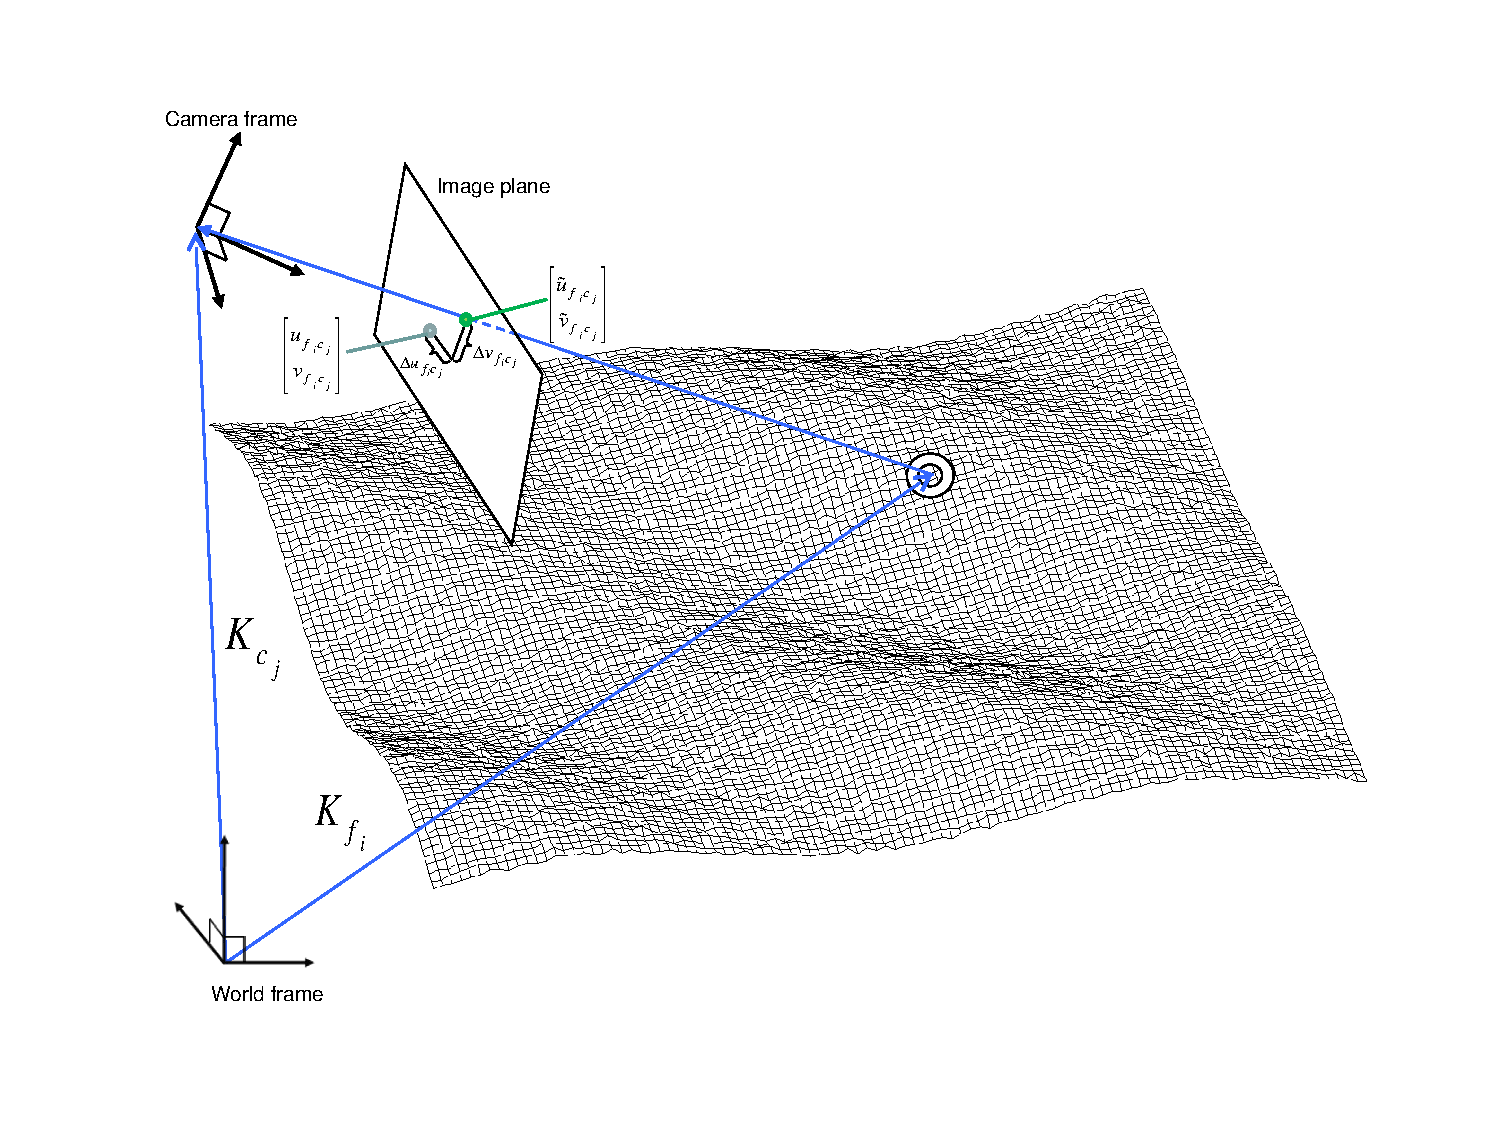
\includegraphics[trim=20mm 20mm 20mm 15mm,clip,width=6in]{images/ba_feature_observation.pdf}
  \end{center}
  \caption{ A feature observation in bundle adjustment, from \citet{moore09} }
  \label{fig:ba_feature}
\end{figure}

Bundle Adjustment in \ac{ISIS} is performed with the \texttt{jigsaw}
executable. It generally follows the method described
in~\cite{triggs00} and determines the best camera parameters that
minimize the projection error given by ${\bf \epsilon} =
\sum_k\sum_j(I_k-I(C_j, X_k))^2$ where $I_k$ are the tie points on the
image plane, $C_j$ are the camera parameters, and $X_k$ are the 3D
positions associated with features $I_k$. $I(C_j, X_k)$ is an image
formation model (i.e. forward projection) for a given camera and 3D
point. To recap, it projects the 3D point, $X_k$, into the camera with
parameters $C_j$. This produces a predicted image location for the 3D
point that is compared against the observed location, $I_k$. It then
reduces this error with the Levenberg-Marquardt algorithm (LMA). Speed
is improved by using sparse methods as described in \citet{hartley04},
\citet{konolige:sparsesparse}, and \citet{cholmod}.

Even though the arithmetic for bundle adjustment sounds clever, there
are faults with the base implementation. Imagine a case where all
cameras and 3D points were collapsed into a single point. If you
evaluate the above cost function, you'll find that the error is indeed
zero. This is not the correct solution if the images were taken
from orbit. Another example is if a translation was applied equally to
all 3D points and camera locations. This again would not affect the
cost function. This fault comes from bundle adjustment's inability to
control the scale and translation of the solution. It will correct the
geometric shape of the problem, yet it cannot guarantee that the solution
will have correct scale and translation.

\ac{ISIS} attempts to fix this problem by adding two additional cost
functions to bundle adjustment. First of which is ${\bf \epsilon} =
\sum_j(C_j^{initial}-C_j)^2$. This constrains camera parameters to
stay relatively close to their initial values. Second, a small handful
of 3D ground control points can be chosen by hand and added to the
error metric as ${\bf \epsilon} = \sum_k(X_k^{gcp}-X_k)^2$ to
constrain these points to known locations in the planetary coordinate
frame. A physical example of a ground control point could be the
location of a lander that has a well known location. \acp{GCP} could also be
hand-picked points against a highly regarded and prior existing map
such as the THEMIS Global Mosaic or the LRO-WAC Global Mosaic.

Like other iterative optimization methods, there are several
conditions that will cause bundle adjustment to terminate. When
updates to parameters become insignificantly small or when the error,
${\bf \epsilon}$, becomes insignificantly small, then the algorithm
has converged and the result is most likely as good as it will get.
However, the algorithm will also terminate when the number of
iterations becomes too large in which case bundle adjustment may or
may not have finished refining the parameters of the cameras.

\subsection{Tutorial: Processing Mars Orbital Camera Imagery}
\label{sec:ba_example}

This tutorial for ISIS's bundle adjustment tools is taken from
\cite{lunokhod:controlnetwork} and \cite{lunokhod:gcp}. These tools
are not a product of NASA nor the authors of Stereo Pipeline. They
were created by USGS and their documentation is available at
\cite{isis:documentation}.

What follows is an example of bundle adjustment using two \ac{MOC}
images of Hrad Vallis. We use images E02/01461 and M01/00115, the same
as used in Chapter~\ref{ch:moc_tutorial}. These images are available from
NASA's \ac{PDS} (the \ac{ISIS} \texttt{mocproc} program will operate
on either the IMQ or IMG format files, we use the \texttt{.imq} below
in the example).  For reference, the following \ac{ISIS} commands are
how to convert the \ac{MOC} images to \ac{ISIS} cubes.

\begin{verbatim}
  ISIS 3> mocproc from=e0201461.imq to=e0201461.cub mapping=no
  ISIS 3> mocproc from=m0100115.imq to=m0100115.cub mapping=no
\end{verbatim}

Note that the resulting images are not map-projected. Bundle
adjustment requires the ability to project arbitrary 3D points into
the camera frame. The process of map-projecting an image dissociates
the camera model from the image. Map-projecting can be perceived as
the generation of a new infinitely large camera sensor that may be
parallel to the surface, a conic shape, or something more
complex. That makes it extremely hard to project a random point into
the camera's original model. The math would follow the transformation
from projection into the camera frame, then projected back down to
surface that ISIS uses, then finally up into the infinitely large
sensor. \texttt{Jigsaw} does not support this and thus does not
operate on map-projected imagery.

Before we can dive into creating our tie-point measurements we must
finish prepping these images. The following commands will add a vector
layer to the cube file that describes its outline on the globe. It
will also create a data file that describes the overlapping sections
between files.

\begin{verbatim}
  ISIS 3> footprintinit from=e0201461.cub
  ISIS 3> footprintinit from=m0100115.cub
  ISIS 3> echo *cub |  xargs -n1 echo > cube.lis
  ISIS 3> findimageoverlaps from=cube.lis overlaplist=overlap.lis
\end{verbatim}

At this point, we are ready to start generating our measurements. This
is a three step process that requires defining a geographic pattern
for the layout of the points on the groups, an automatic registration
pass, and finally a manual clean up of all measurements. Creating the
ground pattern of measurements is performed with \texttt{autoseed}. It
requires a settings file that defines the spacing in meters between
measurements. For this example, write the following text into a
\textit{autoseed.def} file.

\begin{verbatim}
  Group = PolygonSeederAlgorithm
        Name = Grid
        MinimumThickness = 0.01
        MinimumArea = 1
        XSpacing = 1000
        YSpacing = 2000
  End_Group
\end{verbatim}

The minimum thickness defines the minimum ratio between the sides of
the region that can have points applied to it. A choice of 1 would
define a square and anything less defines thinner and thinner
rectangles. The minimum area argument defines the minimum square
meters that must be in an overlap region. The last two are the spacing
in meters between control points. Those values were specifically
chosen for this pair so that about 30 measurements would be produced
from \texttt{autoseed}. Having more control points just makes for more
work later on in this process. Run \texttt{autoseed} with the
following instruction.

\begin{figure}[ht]
  \centering
  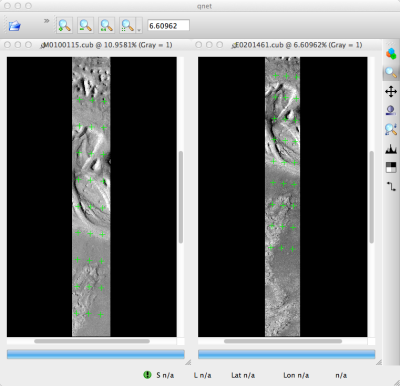
\includegraphics[width=5in]{images/qnet/Qnet_AfterAutoseed_400px.png}
  \caption{A visualization of the features laid out by
    \texttt{autoseed} in \texttt{qnet}. Note that the marks do not
    cover the same features between images. This is due to the poor
    initial spice data for MOC imagery.}
  \label{fig:after_autoseed}
\end{figure}

\begin{verbatim}
  ISIS 3> autoseed fromlist=cube.lis overlaplist=overlap.lis    \
            onet=control.net deffile=autoseed.def networkid=moc \
            pointid=???? description=hrad_vallis
\end{verbatim}

The next step is to perform auto registration of these features
between the two images using \texttt{pointreg}. This program also
requires a settings file that describes how to do the automatic
search. Copy the text box below into a \textit{autoRegTemplate.def}
file.

\begin{verbatim}
   Object = AutoRegistration
    Group = Algorithm
      Name         = MaximumCorrelation
      Tolerance    = 0.7
    EndGroup

    Group = PatternChip
      Samples = 21
      Lines   = 21
      MinimumZScore = 1.5
      ValidPercent = 80
    EndGroup

    Group = SearchChip
      Samples = 75
      Lines   = 1000
    EndGroup
  EndObject
\end{verbatim}

The search chip defines the search range for which \texttt{pointreg}
will look for matching imagery. The pattern chip is simply the kernel
size of the matching template. The search range is specific for this
image pair. The control network result after \texttt{autoseed} had a
large vertical offset in the ball park of 500 px. The large
misalignment dictated the need for the large search in the lines
direction. Use \texttt{qnet} to get an idea for what the pixel shifts
look like in your stereo pair to help you decide on a search range. In
this example, only one measurement failed to match automatically. Here
are the arguments to use in this example of \texttt{pointreg}.

\begin{verbatim}
  ISIS 3> pointreg fromlist=cube.lis cnet=control.net             \
             onet=control_pointreg.net deffile=autoRegTemplate.def
\end{verbatim}

The third step is to manually edit the control and verify the
measurements in \texttt{qnet}. Type \texttt{qnet} in the terminal and
then open \textit{cube.lis} and lastly
\textit{control\_pointreg.net}. From the Control Network Navigator
window, click on the first point listed as \textit{0001}. That opens a
third window called the Qnet Tool. That window will allow you to play
a flip animation that shows alignment of the feature between the two
images. Correcting a measurement is performed by left clicking in the
right image, then clicking \textit{Save Measure}, and finally
finishing by clicking \textit{Save Point}.

In this tutorial, measurement \textit{0025} ended up being
incorrect. Your number may vary if you used different settings than
the above or if MOC spice data has improved since this writing. When
finished, go back to the main Qnet window. Save the final control
network as \textit{control\_qnet.net} by clicking on \textit{File},
and then \textit{Save As}.

\begin{figure}[ht]
  \centering
  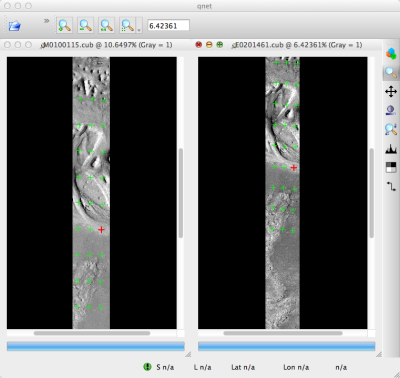
\includegraphics[width=5in]{images/qnet/Qnet_AfterQnetManual_400px.png}
  \caption{A visualization of the features after manual editing in
    \texttt{qnet}. Note that the marks now appear in the same location
    between images.}
  \label{fig:after_manual}
\end{figure}

Once the control network is finished, it is finally time to start
bundle adjustment. Here's what the call to \texttt{jigsaw} looks like:

\begin{verbatim}
  ISIS 3> jigsaw fromlist=cube.lis update=yes twist=no radius=yes \
             cnet=control_qnet.net onet=control_ba.net
\end{verbatim}

The update option defines that we would like to update the camera
pointing, if our bundle adjustment converges. The \textit{twist=no}
says to not solve for the camera rotation about the camera bore. That
property is usually very well known as it is critical for integrating
an image with a line-scan camera. The \textit{radius=yes} means that
the radius of the 3D features can be solved for. Using no will force
the points to use height values from another source, usually LOLA or
MOLA.

The above command will spew out a bunch of diagnostic information from
every iteration of the optimization algorithm. The most important
feature to look at is the \textit{sigma0} value. It represents the mean of
pixel errors in the control network. In our run, the initial error was
1065 px and the final solution had an error of 1.1 px.

Producing a DEM using the newly created camera corrections is the same
as covered in the Tutorial on page \pageref{ch:moc_tutorial}. When using
\texttt{jigsaw}, it modifies a copy of the spice data that is stored
internally to the cube file. Thus when we want to create a DEM using
the correct camera geometry, no extra information needs to be given to
\texttt{stereo} since it is already contained in the file. In the
event a mistake has been made, \texttt{spiceinit} will overwrite the
spice data inside a cube file and provide the original uncorrected
camera pointing.

\begin{verbatim}
  ISIS 3> stereo E0201461.cub M0100115.cub bundled/bundled
\end{verbatim}

%% \subsection{Processing with Ground Control Points}

%% Ground control point files describe a single point in the world
%% that is seen by 1 or more cameras. How they are measured in the
%% first place is up to the user. We use a manual process of comparing
%% each image to a respected map-projected image and then recording
%% the latitude, longitude, and altitude of the point(s). The maps to
%% register against can be anything, but it is recommended to register
%% against a product with a high amount of cartographic stability and
%% accuracy.  For terrestrial work, we would use a \ac{USGS} product
%% that can provide imagery that is registered to LIDAR height
%% measurements.

%% Unlike match files, ground control points must specifically be given
%% to \texttt{isis\_adjust} from the command line, but in no particular
%% order. Ground control point files are written with the extension
%% \texttt{.gcp}. Below is an example of a ground control point file that
%% was created to control a series of Apollo Metric Camera images from
%% several Apollo 15 orbits.

%% \begin{verbatim}
%%     -52.8452 27.2561 1735999 300 300 500
%%     sub4-AS15-M-2086.cub     210.9   3565.0
%%     sub4-AS15-M-2087.cub     1476.9  3579.0
%%     sub4-AS15-M-2088.cub     2798.9  3586.8
%%     sub4-AS15-M-2089.cub     4133.5  3588.6
%%     sub4-AS15-M-2344.cub     906.9   3874.8
%%     sub4-AS15-M-2345.cub     2204.2  3913.9
%%     sub4-AS15-M-2482.cub     939.8   4348.0
%%     sub4-AS15-M-2483.cub     2282.0  4340.7
%%     sub4-AS15-M-2484.cub     3642.1  4330.9
%% \end{verbatim}

%% The first line of a \texttt{.gcp} file is like a header line and
%% is different from the remaining lines.  The first line defines the
%% world location of the ground control point, and the rest of the
%% lines define the image locations of the ground control points. Here
%% are what the columns mean for the first line.

%% \begin{myindentpar}{2cm}
%% \begin{description}
%%   \item[Column 1:] Longitude in degrees
%%   \item[Column 2:] Latitude in degrees
%%   \item[Column 3:] Radius in meters
%%   \item[Column 4:] Sigma (or uncertainty) in meters for Local X axis
%%   \item[Column 5:] Sigma (or uncertainty) in meters for Local Y axis
%%   \item[Column 6:] Sigma (or uncertainty) in meters for Local Z axis
%% \end{description}
%% \end{myindentpar}

%% The other lines describe where this \ac{GCP} is found in each image:

%% \begin{myindentpar}{2cm}
%% \begin{description}
%%   \item[Column 1:] Image name
%%   \item[Column 2:] Sample (X) image measurement
%%   \item[Column 3:] Line (Y) image measurement
%% \end{description}
%% \end{myindentpar}

%% Make a {\tt .gcp} file for every ground control point, then be sure
%% to feed them as an input to {\tt isis\_adjust}. Remember that you
%% can scale the sigma of all ground control points by using the {\tt
%% -\/-gcp-scalar} flag. This can save time by allowing you to make
%% adjustments without needing to edit all of the files individually.
